\documentclass[twoside,11pt]{article}

\usepackage{TechReport_2017_CZ}


\fancyhf{}
\lhead{\color{bgr_DarkBlue}SDR v navigačních systémech}
\rhead{\color{bgr_DarkBlue}Implementace vysílače}

\lfoot{\color{bgr_DarkBlue} v2.0, 2017}
\rfoot{\color{bgr_DarkBlue} Strana \thepage}


\begin{document}

\begin{titlepage}



\center % Center everything on the page

%----------------------------------------------------------------------------------------
%	HEADING SECTIONS
%----------------------------------------------------------------------------------------



%----------------------------------------------------------------------------------------
%	TITLE SECTION
%----------------------------------------------------------------------------------------


{ \huge \bfseries Použití softwarově definovaného rádia v~leteckých navigačních aplikacích.}\\[2in] % Title of your document
\fontsize{17}{12}\textbf{\textcolor{bgr_DarkBlue}{Simulace a implementace vybraných částí vysílače}}\\[4in]
        
%----------------------------------------------------------------------------------------
%	AUTHOR SECTION
%----------------------------------------------------------------------------------------
\begin{minipage}{0.9\textwidth}
\begin{flushleft} \large
\emph{Autor:} Petr \textsc{BOJDA}\\

\emph{Adresa:} Morávka 575, okr. Frýdek-Místek\\
\emph{Dne:} 30. května 2017\\%\today\\
\emph{Verze dokumentu:} 2.0
\end{flushleft}
\end{minipage}

% generates the title

\end{titlepage}

% ********************************** CHAPTER 1 Úvod ***********************************************
% ********************************** CHAPTER 1 source ***********************************************
\section{Úvod}


\marginpar{\textcolor{txt_blue}{Hlavní cíl zprávy}} 
Zpráva vzniká na podnět výzkumného týmu Katedry Leteckých elektrotechnických systémů k podpoře výzkumného úkolu v oblasti terestriálních navigačních systémů s rozprostřeným spektrem. Cílem je nalézt vhodnou strukturu a parametry signálu tak, aby co nejlépe vyhověl požadavkům na celkový systém. V této fázi bude důraz kladen zejména na co nejlepší autokorelační vlastnosti signálu tak, aby bylo dosaženo co nejpřesnější synchronizace, resp. měření časového zpoždění.

\marginpar{\textcolor{txt_blue}{Sekundární cíl zprávy}} 
Dalším důvodem ke vzniku této zprávy je snaha demonstrovat, případně i pomoci s přípravou výuky v oblasti digitálních rádiových systémů. Pozornost je věnována hlavně moderním přístupům k návrhu, analýze, verifikaci a implementaci jednotlivých částí digitálního rádiového systému na bázi softwarově definovaného rádia (SDR). Nedílnou součástí zprávy jsou ucelené bloky softwaru (knihovny a aplikace) vytvořené tak, aby jednak plnily požadovanou funkci v rámci návrhu systému, ale zároveň aby dostatečně srozumitelně demonstrovaly způsob psaní daného typu programu a jeho použití. 

\marginpar{\textcolor{txt_blue}{Použité prostředky}} 
Zpráva vznikla jako komentovaný popis a dokumentace návrhu digitálního rádiového systému. Zahrnuje základní kroky návrhu - simulaci, testování (verifikaci) a nakonec i finální implementaci. Cílovou platformou je SDR, tudíž lze předpokládat, že funkce rádiového systému bude popsána, definována a implementována formou bloků software. Veškeré softwarové nástroje a prostředky použité při zpracování této zprávy jsou v kategorii "Open-Source Software License", zejména BSD licence v případě simulačních nástrojů a GNU GPL v případě implementačních nástrojů. Textová část je editována v systému Latex. Jednotlivé práce byly odvedeny na počítačích s operačním systémem Linux, distribuce Ubuntu. Nebyly použity žádné softwarové nástroje podléhající komerční licenci.

K simulaci je využit systém knihoven v jazyce Python, zejména pak knihovny NumPy, Matplotlib a SciPy. S využitím funkcí těchto knihoven byly vytvořeny knihovny vlastních funkcí ke generování signálů, jejich modulace v základním pásmu (baseband), jejich konverze do vyššího kmitočtového pásma (up-convertor), filtrace, tvarování impulzu s ohledem na minimalizaci mezisymbolové interference při přenosu signálu kanálem s omezeným kmitočtovým pásmem (ISI - Inter-Symbol Interference) a další. Jak bylo uvedeno výše, všechny simulace jsou psány v programovacím jazyce Python.

Prvky digitálního rádiového systému jsou implementovány do SDR E310 firmy Ettus a/nebo s pomocí levného USB přijímače DVB-TV signnálu s čipem RTL2832U. Implementace je ve většině případů provedena pomocí softwarového balíku GNU Radio. Některé části jsou pak implementovány přímo za použití knihovních funkcí výrobce rádia E310, tzv. API funkcí v jazyce C++.

%\lstinputlisting[language=Python]{./ch_01/src/testbed.py}


% ********************************** CHAPTER 2 Simulace ***********************************
% ********************************** CHAPTER 1 source ***********************************************
\section{Struktura digitálního rádiového systému}



\marginpar{\textcolor{txt_blue}{Složení systému}} 
Tato práce se zabývá obecným digitálním rádiovým systémem. V leteckých aplikacích jsou rádiové systémy použity ve třech základních oblastech: komunikační, navigační a přehledové. Podle toho, jaký je primární účel systému, mění se i jeho složení a nastavení parametrů. Společná je jejich základní struktura: 

\begin{itemize}
\item Vysílač
\item Přenosový kanál
\item Přijímač
\end{itemize}

V dalším  budou analyzovány tyto tři komponenty oprostěné od funkcí specifických pro dané oblasti použití. To znamená, že nebude zahrnuto například různé kódování přenášené bitové posloupnosti (zdrojové či kanálové) a podobně. Vstupem vysílače je logický signál. Ten je modulován některou z mnoha digitálních modulací na nosný harmonický signál a anténou vyslán do prostoru. Přenosový kanál reprezentuje souhrnně vliv prostředí (přenosového média) na přenášený signál. Jako příklad je možno jmenovat: přidaný šum, útlum, vícecestné šíření, dopplerův posun, interference, omezení šířky pásma přenášeného signálu a jiné. Zkreslený signál je poté detekován a zpracován pomocí přijímače.


 
\vspace{0.25in}


%%%%%%%%%%%%%%%%%%%%%%%%%%%%%%%%%%%%%%% Popis vysílače %%%%%%%%%%%%%%%%%%%%%%

\subsection{Vysílač}

\marginpar{\textcolor{txt_blue}{Popis struktury vysílače}} 
Struktura vysílače, jak bude v následném textu chápána a analyzována je na obr. \ref{fig_block_Tx}. Vstupní signál $x_b(n)$ je bitovou posloupností nesoucí požadovanou informaci. Blok \textsl{Modulátor BB} přemění -- moduluje vstupní bitovou posloupnost na komplexní signál v základním pásmu (angl. \textsl{baseband}). Signál v základním pásmu $x_{rect}(t)$ pomocí aktuální úrovně své reálné a imaginární složky precizně definuje amplitudu a fázi nosné složky budoucího výstupního signálu vysílače  $x_{RF}(t)$. To je již signál s harmonickou nosnou, na kterou vybranou digitální modulací namodulována bitová posloupnost $x_b(n)$. 

\begin{figure}[ht]
 \begin{minipage}[c]{0.65\textwidth}
   
\tikzstyle{block} = [draw, fill=blue!20, rectangle, 
    minimum height=3em, minimum width=5em]
\tikzstyle{sum} = [draw, fill=blue!20, circle, node distance=1cm]
\tikzstyle{input} = [coordinate]
\tikzstyle{output} = [coordinate]
%\tikzstyle{pinstyle} = [pin edge={to-,thin,black}]

\begin{tikzpicture}[node distance=3cm,auto,>=latex']

    \node [input, name=input] {};
    \node [block, right of=input] (b_A) {Modulátor BB};
	\node [block, right of=b_A,xshift=2cm] (b_B) {Tvarování impulzu};
	\node [block, below of=b_B] (b_C) {Up-Convertor};
	\node [block, left of=b_C,xshift=-2cm] (b_D) {Přenosový kanál};
    \node [output, left of=b_D] (output) {};
 
    \draw [draw,->] (input) -- node {$x_b(n)$} (b_A);
	\draw [draw,->] (b_A) -- node {$x_{rect}(t)$} (b_B);
	\draw [draw,->] (b_B) -- node {$x_{rcos}(t)$} (b_C);
	\draw [draw,->] (b_C) -- node {$x_{RF}(t)$} (b_D);
    \draw [->] (b_D) -- node {$x_{dist}(t)$} (output);

\end{tikzpicture}

 \end{minipage}\hfill
 \begin{minipage}[t]{0.3\textwidth}
  \caption{Základní struktura digitálního rádiového vysílače.\label{fig_block_Tx}}
 \end{minipage}
\end{figure}

\marginpar{\textcolor{txt_blue}{Baseband modulace -- signál v základním pásmu}} 
 SDR (ať už simulované, nebo reálně využívané v této zprávě) používá k transformaci (konverzi) ze základního kmitočtového pásma do pásma nosného kmitočtu (angl. \textsl{passband}) obvod kmitočtové přeměny (tzv. směšovač) \textsl{Up-Convertor} typu kvadraturní modulátor. Tento typ obvodu vyžaduje komplexní vstupní signál v základním pásmu. Komplexní signál v základním pásmu je tvořen reálnou (soufázní, angl. \textsl{In-Phase}) a imaginární (kvadraturní, angl. \textsl{Quadrature}) složkou\footnote{Soufázní složka signálu bývá v technické praxi často označována jako signál I, kvadraturní pak jako Q.}. Blok \textsl{Modulátor BB} tvaruje ze vstupní posloupnosti $x_b(n)$ komplexní $x_{rect}r(t)$ signál, který je charakterizovaný svou tzv. bitovou (symbolovou) rychlostí (angl. \textsl{bitrate})\footnote{V případě \textsl{m-stavové} modulace je poměr bitové rychlosti k rychlosti symbolové dán počtem bitů přenesených v jednom symbolu.} a amplitudou. "\textsl{Modulátor BB}" je již navržen konkrétně pro daný typ výsledné digitální modulace signálu na výstupu vysílače $x_{RF}(t)$. Přicházející bity vstupní posloupnosti $x_b(n)$ jsou nejprve seskupovány podle typu výsledné modulace, viz.:

\begin{itemize}
\item dvoustavová: 1 symbol signálu $x_{rect}(t)$ odpovídá 1 bitu posloupnosti $x_b(n)$, 
\item čtyřstavová: 1 symbol signálu $x_{rect}(t)$ odpovídá 2 bitům posloupnosti $x_b(n)$,
\item osmistavová: 1 symbol signálu $x_{rect}(t)$ odpovídá 3 bitům posloupnosti $x_b(n)$, \ldots
\end{itemize}

Poté jsou seskupené bity tvořící \textsl{m-tice} (angl. \textsl{tuples}) mapovány na patřičnou reprezentaci pomocí komplexního signálu $x_{rect}(t)$. Pro každou kombinaci bitů symbolu je definována i kombinace úrovní\footnote{kvantizační úroveň může být dána přímo napětím, nebo vyjádřena jen číselně. To záleží na aktuální podobě obvodu Up-konvertoru. Někdy je vyžadován vstupní signál v základním pásmu, tzv. I a Q v analogové podobě. Moderní integrované obvody provádějící konverzi však často obsahují na vstupu dva DA převodníky a signál v základním pásmu je na ně přiváděn ve formě diskrétních I a Q vzorků.} soufázní a kvadraturní složky signálu $x_{rect}(t)$. Jedním ze základních parametrů digitálních rádiových systémů je i požadovaná přenosová \textsl{bitová} (angl. \textsl{bitrate}) a z ní odvozená \textsl{symbolová} (angl. \textsl{symbol--rate}) rychlost. Symbolová rychlost definuje dobu trvání jednoho symbolu (impulzu) $T_S$.

\begin{figure}[ht]
 \begin{minipage}[c]{0.65\textwidth}
  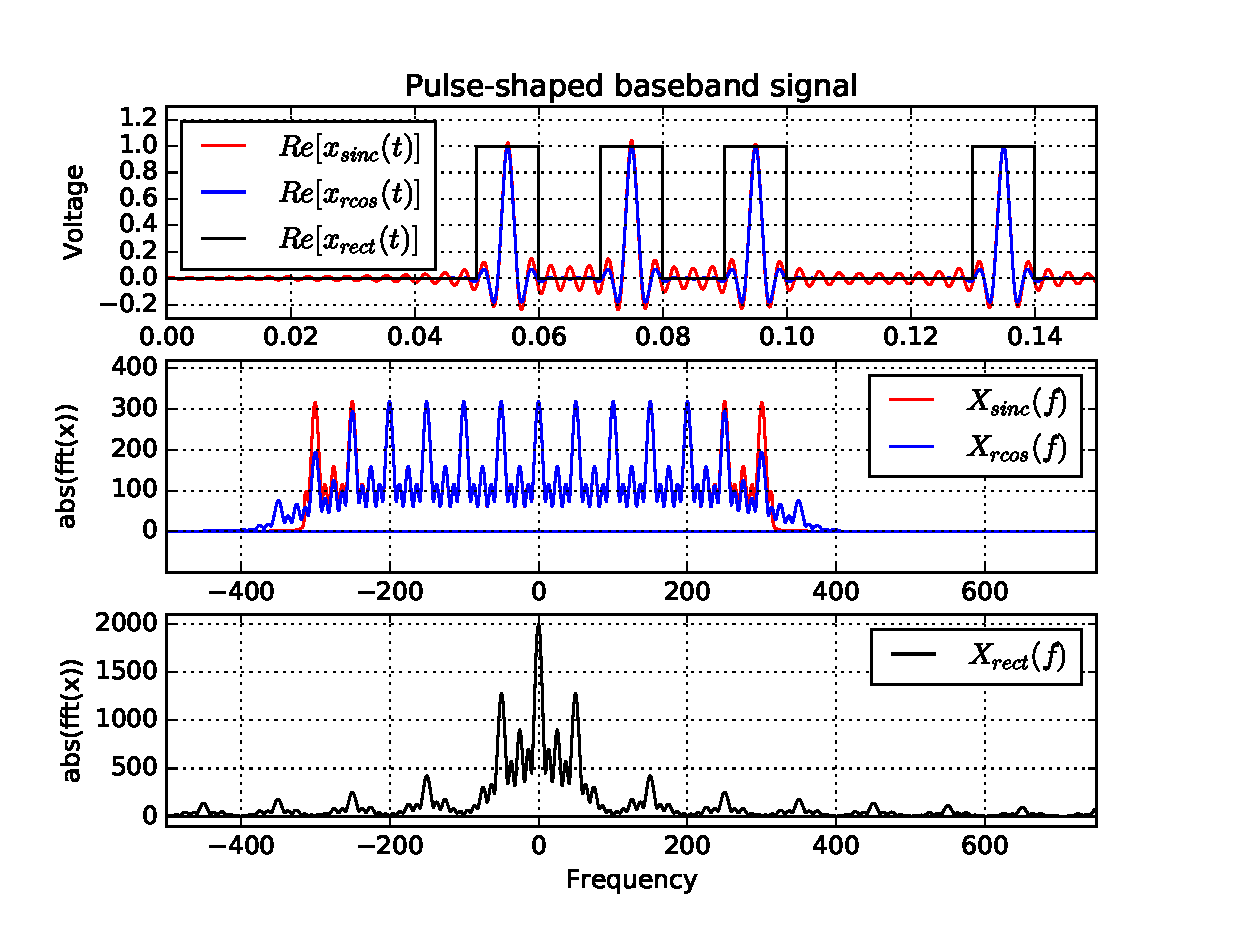
\includegraphics[width=4in]{./ch_02/img/Pulse_shaping.eps}
 \end{minipage}\hfill
 \begin{minipage}[t]{0.3\textwidth}
  \caption{Příklad tvarování impulzu signálu v základním pásmu. Kvůli jednoduchosti je znázorněná pouze jedna (uvažujme například, že reálná - symfázní) složka komplexního signálu.\label{fig_pulse_shaped}}
 \end{minipage}
\end{figure}

\marginpar{\textcolor{txt_blue}{Tvarování pulzu}}
Za blokem \textsl{Modulátoru BB} jsou přechody mezi jednotlivými symboly signálu $x_{rect}(t)$\footnote{U komplexního signálu v základním pásmu se už nehovoří o "bitech", ale o "symbolech". Přestože v tuto chvíli pojem "symbolu" ještě není precizně definován, je kvůli správnosti výkladu použit. Nicméně, v případě dvoustavových modulací obsahuje symbol jeden datový bit. Proto je možné setkat se někdy v technické literatuře s pojmem "bit" i v případě \textsl{baseband} signálu.} ideálně strmé, viz obr. \ref{fig_pulse_shaped}. Signál v základním pásmu (\textsl{baseband} signál) má v tuto chvíli podobu ideálních obdélníkových impulzů. Obdélníkový průběh je v reálných podmínkách nevýhodný. Skutečné přenosové kanály značně omezují kmitočtové spektrum přenášených signálů a potlačují některé kmitočty. Zjednodušeně lze jejich chování modelovat filtry typu dolní nebo pásmová propust\footnote{V angl. psané literatuře jsou označovány jako "\textsl{bandlimited channels}"}. Pro soudobé systémy pracující s vysokými bitovými (symbolovými) rychlostmi by nepredikovatelné zkreslení impulzu jednotlivých symbolů představovalo vážný problém při detekci a následném zpracování signálu v přijímači. Proto blok \textsl{Tvarování impulzu} kontrolovaně omezí pásmo signálu $x_{rect}(t)$ tím, že tvaruje jednotlivé impulzy symbolů podle vhodných matematických funkcí. Teoreticky je jich používáno více (\textsl{gauss}, \textsl{sinc}, \ldots), prakticky jsou používány funkce \textsl{raised-cosine} (ve zkratce \textsl{rcos}). V podstatě se jedná o "utlumenou" funkci sinc (angl. \textsl{damped sinc}). Výstupem bloku "\textsl{Tvarování impulzu}" je tedy signál $x_{rcos}(t)$, jehož kmitočtové spektrum je na rozdíl od signálu $x_{rect}(t)$ ohraničené a definované už v době návrhu systému. Signál $x_{rect}(t)$ s ideálně obdélníkovým průběhem, signál $x_{rcos}(t)$, kde je impulz tvarován funkcí raised-cosine a nakonec i signál $x_{sinc}(t)$ s impulzem ve tvaru funkce sinc spolu se svými kmitočtovými spektry jsou prezentovány na obrázku \ref{fig_pulse_shaped}. 



\marginpar{\textcolor{txt_blue}{Up-Convertor, Transformace do pásma VF}}
Komplexní signál $x_{rcos}(t)$ je připraven k transformaci (ke konverzi) do kmitočtového pásma vhodného pro daný systém. Většina SDR dnes využívá obvod \textsl{kvadraturní modulátor}. Tento typ modulátoru (často pojmenovávaného anglicky \textsl{Up-Convertor}) umožňuje obrovskou flexibilitu celého rádia. Je jedním z hlavních stavebních prvků SDR a příčinou "softwarového" přístupu k tvarování signálu rádia. Jde o to, že nezměněná hardwarová struktura může vygenerovat signál $x_{RF}(t)$ s takřka libovolnou digitální modulací. Záleží jen na tom, jak bude vypadat komplexní signál v základním pásmu $x_{rcos}(t)$. Ten, pomocí své reálné složky $Re[x_{rcos}(t)]$ a imaginární složky $Im[x_{rcos}(t)]$ přesně určuje fázi $\phi_{RF}(t)$ a amplitudu výsledného signálu $x_{RF}(t)$. Obrázek \ref{fig_quad_principle} demonstruje tento princip. Zde uvažujeme pouze digitální modulace s konstantní amplitudou nosného signálu. U nich je manipulováno jen s fází $\phi_{RF}(t)$\footnote{Skupina modulací manipulujících s fází (v angl. \textsl{PSK}, čili \textsl{phase shift keying})} nosného harmonického signálu.
 
\begin{figure}[ht]
 \begin{minipage}[c]{0.65\textwidth}
  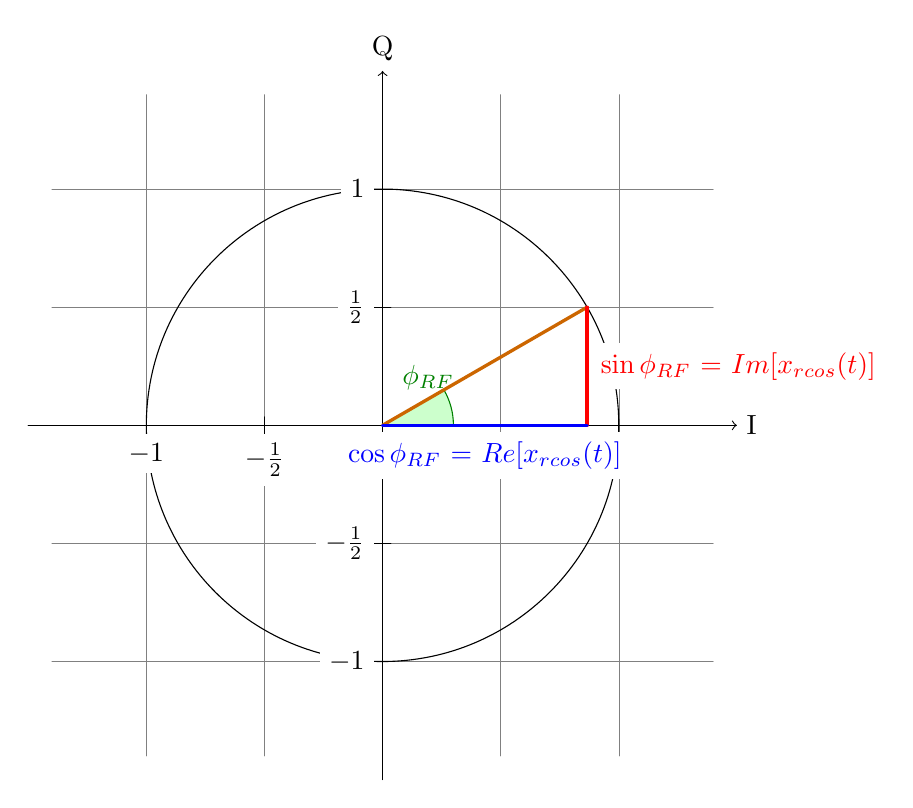
\begin{tikzpicture}[scale=3,cap=round]
  % Local definitions
  \def\costhirty{0.8660256}

  % Colors
  \colorlet{anglecolor}{green!50!black}
  \colorlet{sincolor}{red}
  \colorlet{amplcolor}{orange!80!black}
  \colorlet{coscolor}{blue}

  % Styles
  \tikzstyle{axes}=[]
  \tikzstyle{important line}=[very thick]
  \tikzstyle{information text}=[rounded corners,fill=red!10,inner sep=1ex]

  % The graphic
  \draw[style=help lines,step=0.5cm] (-1.4,-1.4) grid (1.4,1.4);

  \draw (0,0) circle (1cm);

  \begin{scope}[style=axes]
    \draw[->] (-1.5,0) -- (1.5,0) node[right] {I};
    \draw[->] (0,-1.5) -- (0,1.5) node[above] {Q};

    \foreach \x/\xtext in {-1, -.5/-\frac{1}{2}, 1}
      \draw[xshift=\x cm] (0pt,1pt) -- (0pt,-1pt) node[below,fill=white]
            {$\xtext$};

    \foreach \y/\ytext in {-1, -.5/-\frac{1}{2}, .5/\frac{1}{2}, 1}
      \draw[yshift=\y cm] (1pt,0pt) -- (-1pt,0pt) node[left,fill=white]
            {$\ytext$};
  \end{scope}

  \filldraw[fill=green!20,draw=anglecolor] (0,0) -- (3mm,0pt) arc(0:30:3mm);
  \draw (15:2mm) node[above=5pt,anglecolor] {$\phi_{RF}$};
  
  \draw [style=important line,amplcolor]
	(0,0) -- (30:1cm);

  \draw[style=important line,sincolor]
    (30:1cm) -- node[right=1pt,fill=white] {$\sin \phi_{RF}$ = $Im[x_{rcos}(t)]$} +(0,-.5);

  \draw[style=important line,coscolor]
    (0,0) -- node[below=2pt,fill=white] {$\cos \phi_{RF}$ = $Re[x_{rcos}(t)]$} (\costhirty,0);

 
\end{tikzpicture}

 \end{minipage}\hfill
 \begin{minipage}[t]{0.3\textwidth}
  \caption{Princip kvadraturní modulace. Význam symfázní a kvadraturní složky signálu základního pásma.\label{fig_quad_principle}}
 \end{minipage}
\end{figure}


Díky nízkým kmitočtům signálů základního pásma je možné k jejich tvarování využít procesorů (často obsahujících podpůrné struktury pro číslicové zpracování signálů) a tím pádem lze jejich strukturu i parametry určovat softwarem v procesoru. Přeneseně tedy software procesoru tvaruje (definuje) vysokofrekvenční signál na výstupu vysílače $x_{RF}(t)$.





% ********************************** CHAPTER 3 Realizace ***********************
% ********************************** CHAPTER 3 source ***********************************************




%%%%%%%%%%%%%%%%%%%%%%%%%%%%%%%%%%%%%%%%%%%%%%%%%%%%%%%%
\section{Teoretický popis funkce vysílače} %%%%%%%%%%%%%%%%%%%%%%%%%%%%%%%%%%%%

Předpokládejme, že systém bude vysílat předem známou -- definovanou posloupnost bitů: $b(n)$ 
\begin{equation}
 b(n) = {b_0,b_1,\ldots,b_N} \label{eq:bseq}
\end{equation}
Známe jednak celkovou délku posloupnosti -- $N$ bitů a také hodnotu každého z bitů posloupnosti $b(n)$, přičemž $n$ je z oboru přirozených čísel. 


%%%%%%%%%%%%%%%%%%%%%%%%%%%%%%%% Modulation
\subsection{Moduační schéma}
\marginpar{\textcolor{txt_blue}{M-stavová modulace}}
Použita bude jednoduchá digitální modulace bez paměti (\textsl{angl.} memoryless), kdy je posloupnost bitů $b(n)$ mapována na jednotlivé symboly z M-prvkové množiny (\textsl{v angl. literatuře} M-ary mapping schema). Zvolená modulace je potom pojmenováne podle počtu dostupných symbolů "M-stavová". Podrobněji viz např. \cite{lathi2009}, \cite{proakis2007} nebo jiná literatura věnující se základům digitální modulace signálů. Posloupnost $b(n)$ je tudíž rozděnena na skupinky bitů o délce $k$, kde  
\begin{equation}
 k = \log_2M.  \label{eq:kfromM}
\end{equation}
Potom se z posloupnosti bitů $b(n)$, viz rovnice (\ref{eq:bseq}), stává posloupnost symbolů $a(l)$
\begin{equation}
 a(l) = {a_0,a_1,\ldots,a_L} \label{eq:sseq}
\end{equation}
Délka posloupnosti symbolů je $L$, kdy $L=\frac{N}{k}$.

\marginpar{\textcolor{txt_blue}{Bandpass signál}}
Každý \textsl{symbol} $a(l)$, který je tvořen skupinkou $k$ bitů je mapován na jeden z $M$ možných signálů $s_m(t)$ (\textsl{angl.} waveforms). 
\begin{equation}
 s_m(t), 1 \leq m \leq 2^k.  \label{eq:waveforms}
\end{equation}

Jedná se o harmonické signály tzv. vysokofrekvenční (VF), tedy fakticky o signály v podobě, v jaké budou vysílány anténou vysílače (\textsl{angl.} bandpass). Ty jsou charakteristické (a jedinečné) svou amplitudou, fází nebo svým kmitočtem, podle typu modulace. 

V této práci se budeme zabývat převážně signály, u nichž je modulovaná jejich fáze (\textsl{angl.}  phase--type of modulation). Podle \cite{proakis2007} je takový signál analyticky vyjádřen:
\begin{equation}
 s_m(t) = h(t)\cdot e^{j\frac{2\pi (m-1)}{M}} \cdot e^{j2\pi f_c t}.  \label{eq:waveformsBP}
\end{equation}

V tuto chvíli je možné $h(t)$ považovat za konstantu, která se v průběhu trvání jednoho symbolu nemění. Prostřední člen, který charakterizuje daný symbol, vyjádříme v exponenciálním tvaru:
\begin{equation}
 e^{j\frac{2\pi (m-1)}{M}} = \cos(2\pi \frac{m-1}{M}) + j\sin(2\pi \frac{m-1}{M}). \label{eq:waveformsBB00}
\end{equation}

\marginpar{\textcolor{txt_blue}{Baseband signál}}
Jak bylo naznačeno v předchozí kapitole, signály zastupující jednotlivé symboly, tedy \textsl{bandpass} signály mohou být reprezentovány jinými - nízkofrekvenčními signály tzv. základního pásma (\textsl{angl.} baseband). Ten je složen ze symfázní složky (\textsl{angl} in-phase) $s_m^I(t)$ a kvadraturní složky (\textsl{angl.} quadrature) $s_m^Q(t)$ podle:
\begin{equation}
 s_m^I(t) = h(t) \cdot \cos(2\pi \frac{m-1}{M}), \label{eq:waveformsI}
\end{equation}
\begin{equation}
 s_m^Q(t) = h(t) \cdot \sin(2\pi \frac{m-1}{M}). \label{eq:waveformsQ}
\end{equation}

Transformace signálu základního pásma na signál VF je realizována pomocí kvadraturního modulátoru (\textsl{angl.} quadrature modulation), viz např. \cite{proakis2007}. 


\subsection{Tvarování impulzu}
Každý ze symbolů posloupnosti $a(l)$ je vysílán po omezenou dobu. Po dobu trvání toho symbolu je vysílán patřičný signál $s_m$, který je v našem případě harmonický signál s příslušnou fází. V dalším textu budou tyto časové úseky nazývány v souladu s zaběhnutou terminologií impulzy. 

Pokud je, jak jsme doposud uvažovali, hodnota $h(t)$ po dobu celého jednoho impulzu konstantní, je okamžitá úroveň signálu základního pásma (jeho I a Q složky) dána hodnotou $m$, viz rovnice (\ref{eq:waveformsI}) a (\ref{eq:waveformsQ}). Pak mluvíme o obdélníkových impulzech (\textsl{angl} rectangular).

Z toho je zřejmé, že funkce $h(t)$ definuje tvar použitého impulzu. Jak bylo již zmíněno v úvodní části, není použití obdélníkových impulzů vždy výhodné vzhledem k jejich nekonečně širokému kmitočtovému spektru. Je běžnou praxí použít jiné -- výhodnější -- funkce pro $h(t)$ než je konstanta, a to například funkci \textsl{raised--cosine}:
 \begin{equation}
 h(t) =  \frac{\sin(\frac{\pi t}{T})}{\frac{\pi t}{T}}\cdot \frac{\cos(\pi \beta \frac{t}{T})}{1-4 \beta^2 (\frac{t}{T})^2}, \label{eq:pulseRC}
\end{equation}
kde $\beta$, z intervalu $0\leq \beta \leq 1$, je tzv. \textsl{roll-off} faktor. Detailněji viz \cite{lathi2009} nebo \cite{proakis2007}. Raised--cosine pulzy pro různé hodnoty $\beta$ jsou znázorněny na obr. \ref{fig:pulse_RCbeta}. Vězte, že pokud $\beta = 0$ potom $h(t)$ přechází na funkci $sinc(\pi t / T)$.

\begin{figure}[!t]
  \centering
  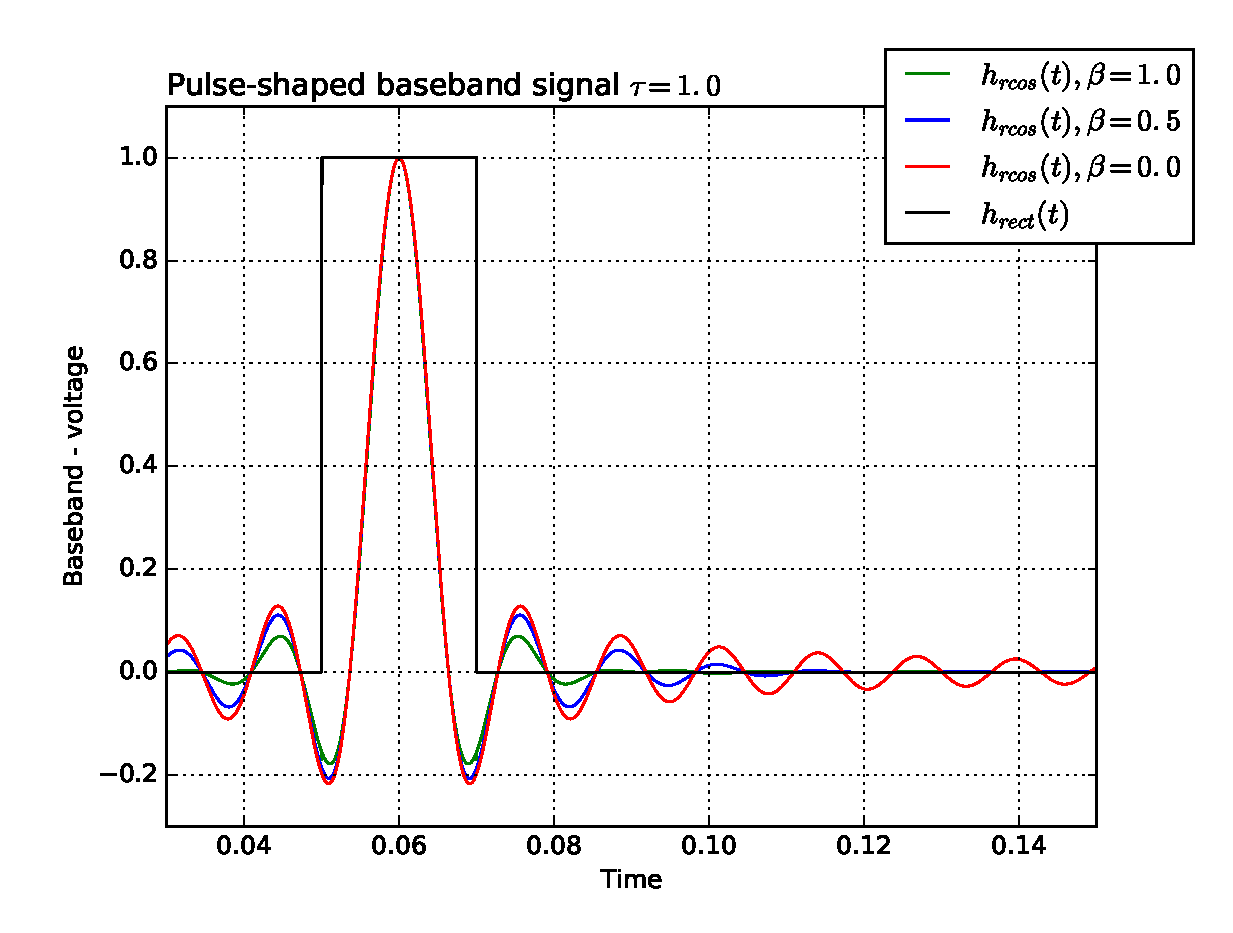
\includegraphics[width=3.5in]{./ch_03/img/Pulse_shaping_1.eps}
  \hfil
  \caption{Raised-cosine impulzy s rozdílnou hodnotou roll-off faktoru $\beta$.\label{fig:pulse_RCbeta}}
\end{figure}

%%%%%%%%%%%%%%%%%%%%%%%%%%%%%%%%%%%%% Timing
\subsection{Popis časových souvislostí signálu s tvarovaným impulzem}
Každý ze signálů $s_m(t)$ je vysílán po dobu trvání jednoho symbolu $T_s$ (\textsl{angl.} symbol interval). Odtud také symbolová rychlost $R_s$ (\textsl{angl.} symbol rate): 
\begin{equation}
 R_s = \frac{1}{T_s}  \label{eq:symrate}
\end{equation}

Potom $T_s$ definuje délku trvání impulzu a každý ze signálů $s_m(t)$ je vysílán uvnitř příslušného symbolového intervalu $T_s$ s patřičnou hodnotou parametru $m$. Tvarovací funkce  $h(t)$ z rovnice. (\ref{eq:pulseRC}) se tudíž mění na:
 \begin{equation}
 h(t-lT_s) =  \frac{\sin(\frac{\pi (t-lT_s)}{T_s})}{\frac{\pi (t-lT_s)}{T_s}}\cdot \frac{\cos(\pi \beta \frac{(t-lT_s)}{T_s})}{1-4 \beta^2 (\frac{(t-lT_s)}{T_s})^2}, \label{eq:pulseRCTs}
\end{equation}
kde $l$ značí pořadové číslo aktuálního symbolu v rámci posloupnosti $a(l)$.

Impuls tohoto tvaru potom splňuje Nyquistovo kritérium, viz \cite{proakis2007}, a nedochází k mezisymbolové interferenci (\textsl{angl} inter--symbol interference) a k nejednoznačnosti při detekci a identifikaci symbolu v přijímači.

Signál základního pásma pro příslušný $l$-tý symbol posloupnosti $a(l)$, potom z rovnice (\ref{eq:sseq}) je dán: 
\begin{equation}
 s_{m,l}^I(t) = h(t-lT_s) \cdot \cos(2\pi \frac{m_l-1}{M}), \label{eq:sigBBI}
\end{equation}
\begin{equation}
 s_{m,l}^Q(t) = h(t-lT_s) \cdot \sin(2\pi \frac{m_l-1}{M}). \label{eq:sigBBQ}
\end{equation}





% ********************************** CHAPTER 3 Realizace ***********************
% ********************************** CHAPTER 4 source ***********************************************
\section{Generátor rádiového signálu}

Z úvodní části tohoto textu a z obrázku \ref{fig_block_Tx} je patrno několik stupňů -- fází, ze kterých se celý proces generování rádiového signálu skládá. Uvažujme, že vstupem je posloupnost, viz rovnice (\ref{eq:bseq}). V první řadě jde o formování požadovaných n-tic bitů přenášené bitové posloupnosti $b(n)$, podle zvoleného počtu stavů modulace $M$. Každá z n-tic bitů definuje hodnotu patřičného symbolu. Hodnotu symbolu je potřeba "namapovat" na patřičnou podobu složek signálu základního pásma a poté složky I a Q, tedy $s_m^I(t)$ a $s_m^Q(t)$, podle rovnic (\ref{eq:waveformsI}) a (\ref{eq:waveformsQ}) vygenerovat.



\marginpar{\textcolor{txt_blue}{up-convertor}} 
V digitálním rádiovém systému slouží blok "Up-Convertor" k transformaci připraveného signálu v základním pásmu (baseband) do kmitočtového pásma vhodného k rádiovému přenosu. řekněme, že daný krok lze nazvat i "modulací nosné".

V tomto projektu bude vytvořen Up-convertor pro účely simulace. Ve vlastní hardwarové implementaci slouží k přeměně samotné rádio, čili fyzicky RF-frontend.


%%%%%%%%%%%%%%%%%%%%%%%%%%%%%%%%%%%%%%%% Diff Equation %%%%%%%%%%%%%%%%%%%%%%%%%%%%%%%%%%%%%%%%%%%%
\subsection{Realizace Up-convertoru - Python}
\marginpar{\textcolor{txt_blue}{Rozbor}} 
Let's start with a time-domain first to derive the differential equation from a \textsl{free-body diagram}. We will use the second Newton's law, setting the mass $M=0$.


\subsection{Způsob generování}

\subsubsection {Přímý generátor}

\subsubsection {Root raised -- cosine filtr}


%%%%%%%%%%%%%%%%%%%%%%%%%%%%%%%%%%%%%%%%%% Time Response %%%%%%%%%%%%%%%%%%%%%%%%%%%%%%%%%%%%%%%%%%%%
\subsection{Použití bloku USRP v GNU Radio}
We are required to derive both natural and step response.


\lstinputlisting[language=Python, caption={Mapování bitové posloupnosti} ,label=lst_recttr]{./ch_04/src/constallation_mappers.py}



% ********************************** CHAPTER 3 Realizace ***********************
% ********************************** CHAPTER 5 source ***********************************************
\section{Simulace - popis vytvořených funkcí}

Veškeré simulace byly vytvořeny v jazyce Python, variantě 3.5.2. s využitím nástrojů knihoven Matplotlib 1.5.3, NumPy 1.11.1 a SciPy 0.18.1, vše instalováno v rámci balíku Anaconda 4.2.0. Simulace byly napsány, vyzkoušeny a provozovány na počítači s operačním systémem Linux Ubuntu 16.04.

Vytvořené funkce simulací jsou sdruženy do několika samostatných souborů s koncovkou \texttt{.py} a umístěné v podadresářích uvnitř samostatného adresáře \texttt{numpy}. Členění do podadresářů je podle logické a funkční příslušnosti. Dále hlavní adresář \texttt{numpy} obsahuje řadu příkladů použití simulačních funkcí.

Funkce ze souborů ve vnořených adresářích lze využít až poté, co jsou do skriptu hlavní úrovně importovány\footnote{Toto je pochopitelně dokumentovanou vlastností jazyka Python. Zde je tento fakt zmíněn pouze jako připomínka.}. 

\subsection{Generátory signálu}

Funkce zde popsané jsou umístěny v podadresáři \texttt{siggens}. Patří k základním prostředkům modulací -- generují signál požadovaného tvaru a parametrů a to jak v podobě základní (jediný, neopakující se impulz), tak i ve variantě opakujících se impulzů obsahujících kód. 

\subsubsection{Jednoduché impulzy}
Funkce, které byly vytvořeny proto, aby generovaly jediný a neopakující se impulz jsou sdruženy v souboru \texttt{one\_pulse.py}. Mohou sloužit jednak k prezentaci impulzu daného tvaru a jeho vlastností, zároveň jsou ale základem pro funkce, které spojují jednotlivé imulzy do jejich posloupností.

\paragraph{Funkce \texttt{rect\_p} - obdélníkový impulz}
Funkce, viz. listing \ref{lst_rectp}, generuje jednoduchý obdélníkový impulz. Vstupními parametry jsou $t_{START}$ a $t_{END}$, tedy okamžik začátku a konce impulzu v rámci časové osy $t$. Výstupem funkce je vektor $p$ vzorků impulzu odpovídajících vzorkovacím okmžikům definovaných vstupním vektorem $t$.

\lstinputlisting[language=Python, caption={Generátor jednorázového obdélníkového impulzu} ,label=lst_rectp]{./ch_05/src/rect.py}

\paragraph{Funkce \texttt{sinc\_p} - $sinc(x)$ impulz}
Funkce, viz. listing \ref{lst_sincp}, generuje jednoduchý sinc impulz. Vstupními parametry jsou $t_{0}$ a $T_{B}$, tedy střed impulzu v rámci časové osy $t$ a šířka hlavního laloku $T_B$. Výstupem funkce je vektor $p$ vzorků impulzu odpovídajících vzorkovacím okmžikům definovaných vstupním vektorem $t$.

\lstinputlisting[language=Python, caption={Generátor jednorázového impulzu tvaru $\frac{\sin(x)}{x}$} ,label=lst_sincp]{./ch_05/src/sinc.py}

\paragraph{Funkce \texttt{rcos\_p} - Raised--cosine impulz}
Funkce, viz. listing \ref{lst_rcosp}, generuje jednoduchý raised--cosine impulz. Vstupními parametry jsou $t_{0}$ a $T_{B}$, tedy střed impulzu v rámci časové osy $t$ a šířka hlavního laloku $T_B$. Výstupem funkce je vektor $p$ vzorků impulzu odpovídajících vzorkovacím okmžikům definovaných vstupním vektorem $t$.

\lstinputlisting[language=Python, caption={Generátor jednorázového impulzu tvaru raised-cosine} ,label=lst_rcosp]{./ch_05/src/rcos.py}

\subsubsection{Posloupnosti impulzů}

Funkce, které byly vytvořeny proto, aby generovaly posloupnost impulzů různého tvaru jsou sdruženy v souboru \texttt{train\_pulse.py}. Jsou napsány tak, aby jednak generovaly impulz požadovaného tvaru několikrát opakovaně v průběhu časové osy cané vektorem $t$. Dále mohou zahrnout i kódování - impulz je nebo není na daném časovém úseku přítomen, podle toho, je-li příslušný bit kódové posloupnosti roven logické jedničce nebo nule. 

\paragraph{Funkce \texttt{rect\_tr} - obdélníkový impulz}
Funkce, viz. listing \ref{lst_recttr}, generuje posloupnost obdélníkových impulzů. Vstupními parametry jsou délka impulzu $t_{p}$, délka mezery mezi impulzy $t_{s}$, a zpoždění celé posloupnosti -- mezera mezi začátkem časové osy $t$ a začátkem prvního impulzu. Dále je vstupem vektor logických hodnot $code$. Ten určuje jednak kódovou posloupnost -- tzn. přítomnost nebo nepřítomnost daného impulzu v rámci celé řady impulzů. Dále počet bitů posloupnosti $code$ určuje počet impulzů výsledného signálu.

Výstupem funkce je vektor $x$ vzorků impulzů odpovídajících vzorkovacím okmžikům definovaných vstupním vektorem $t$.

\lstinputlisting[language=Python, caption={Generátor posloupnosti obdélníkových impulzů} ,label=lst_recttr]{./ch_05/src/TR_rect.py}

\paragraph{Funkce \texttt{sinc\_tr} - $sinc(x)$ impulz}
Funkce, viz. listing \ref{lst_sinctr}, generuje posloupnost impulzů $sinc(x)$. Vstupními parametry jsou délka impulzu $t_{p}$, délka mezery mezi impulzy $t_{s}$, a zpoždění celé posloupnosti -- mezera mezi začátkem časové osy $t$ a středem prvního impulzu. Dále je vstupem vektor logických hodnot $code$. Ten určuje jednak kódovou posloupnost -- tzn. přítomnost nebo nepřítomnost daného impulzu v rámci celé řady impulzů. Dále počet bitů posloupnosti $code$ určuje počet impulzů výsledného signálu.

Parametr $pw$ je specifický pro tvar impulzu $sinc$. Určuje délku hlavního laloku funkce $sinc(x)$ uvnitř celého pulzu $t_p$. Jestliže parametr $t_p$ můžeme nastavit podle bitové rychlosti \textsl{bitrate}, potom samotný $sinc(x)$ impulz může být v rámci jednoho bitu kratší - užší.

Výstupem funkce je vektor $x$ vzorků impulzů odpovídajících vzorkovacím okmžikům definovaných vstupním vektorem $t$.

\lstinputlisting[language=Python, caption={Generátor posloupnosti impulzů $\frac{\sin(x)}{x}$} ,label=lst_sinctr]{./ch_05/src/TR_sinc.py}

\paragraph{Funkce \texttt{rcos\_tr} - Raised--cosine impulz}
Funkce, viz. listing \ref{lst_rcostr}, generuje posloupnost impulzů raised--cosine. Vstupními parametry jsou délka hlavního laloku impulzu $t_{p}$, délka mezery mezi impulzy $t_{s}$, a zpoždění celé posloupnosti -- mezera mezi začátkem časové osy $t$ a středem prvního impulzu. Dále je vstupem vektor logických hodnot $code$. Ten určuje jednak kódovou posloupnost -- tzn. přítomnost nebo nepřítomnost daného impulzu v rámci celé řady impulzů. Dále počet bitů posloupnosti $code$ určuje počet impulzů výsledného signálu.

Parametr $pw$ je jako v případě $sinc$ impulzu specifický pro tvar impulzu raised--cosine. Určuje délku hlavního laloku funkce $sinc(x)$ uvnitř celého pulzu $t_p$. Jestliže parametr $t_p$ můžeme nastavit podle bitové rychlosti \textsl{bitrate}, potom samotný $sinc(x)$ impulz může být v rámci jednoho bitu kratší - užší.

Parametr $alpha$ udává tzv. roll--off faktor funkce raised--cosine.

Výstupem funkce je vektor $x$ vzorků impulzů odpovídajících vzorkovacím okmžikům definovaných vstupním vektorem $t$.

\lstinputlisting[language=Python, caption={Generátor posloupnosti raised--cosine impulzů},label=lst_rcostr]{./ch_05/src/TR_rcos.py}

\begin{boxit}
Důležité: Parametr $t_d$ znamená u posloupnosti obdélníkových impulzů zpoždění posloupnosti vzhledem k náběžné hraně prvního pulzu, u posloupností impulzů tvaru $sinc(x)$ a raised--cosine vzhledem je ke středu hlavního laloku. To je potřeba respektovat, pokud se posloupnosti umisťují na časové ose společně.
\end{boxit}

\subsubsection{Generátory pseudonáhodných posloupností}
Funkce, které byly vytvořeny proto, aby generovaly posloupnosti bitů --- generátory kódových a pseudonáhodných posloupností --- jsou sdruženy v souboru \texttt{PRN\_bitstreams.py}. Tyto funkce jsou vhodné jednak k testování digitálních rádiových systémů a potom k rozprostření kmitočtového spektra v systémech typu DSSS (z angl. \textsl{Direct Sequence Spread Spectrum}). 

\paragraph{\texttt{tri\_seq}: Tří--bitový SSRG.}
Funkce, viz. listing \ref{lst_triseq}, generuje bitovou posloupnost pomocí posuvného registru se zavedenými několika zpětnými vazbami SSRG\footnote{z angl. \textsl{Simple Shift Register Generator}}. V tomto konkrétním případě je použit generátor ve Fibonacciho tvaru s tří--bitovým registrem. Prvním vstupem funkce je parametr \texttt{init\_reg} logický vektor (3 bity), který určuje počáteční stav registru před startem procesu generování posloupnosti. Druhým vstupním parametrem je opět tříbitový logický vektor \texttt{fb\_reg}, který definuje zpětné vazby posuvného registru. Logická "0" v tomto vektoru znamená, že zpětná vazba není z daného bitu posuvného registru odvadana. Naopak logická "1" indikuje přítomnost zpětné vazby z příslušného bitu registru.

Výstupem funkce je 10-ti bitový vektor logických hodnot - vygenerovaná bitová posloupnost.

\lstinputlisting[language=Python, caption={Generátor jednoduché posloupnosti. 3-bitový SSRG, generována je posloupnost 10-ti bitů.} ,label=lst_triseq]{./ch_05/src/tri_seq.py}

\paragraph{\texttt{gold\_seq}: Generátor Goldova kódu.}
Funkce, viz. listing \ref{lst_goldseq}, generuje Goldovu pseudonáhodnou bitovou posloupnost, tzv. Goldův kód. Jsou použity dva 10--bitové posuvné registry se zavedenými vlastními několika zpětnými vazbami a se dvěma vazbami \textsl{vzájemnými}. Vzájemné vazby zabezpečují navázání registrů a spojení dvou nezávislých posloupností do jedné výsledné. Rozmístění vlastních zpětných vazeb jednotlivých registrů, stejně jako jejich počáteční stavy,  jsou v souladu se standardem družicového navigačního systému GPS tak, aby generované posloupnosti odpovídaly posloupnostem použitým v tomto systému.   

Prvními dvěma vstupními parametry jsou umístění \textsl{vzájemných} vazeb \texttt{x1} a \texttt{x2}. Jedná se o celá čísla v rozsahu 0--9, která definují číslo bitu posuvného registru, z nějž je vazba odvedena\footnote{Jednotlivé kombinace \texttt{x1} a \texttt{x2} produkují unikátní posloupnost. Standard popisující systém GPS precizně definuje konkrétní kombinace pro kódy petřící jednotlivým družicím a jiným typům vysílačů v systému (např. družice SBAS, pseudolity a jiné)}.  Třetím vstupním parametrem je opět celé číslo \texttt{N\_codes}, které určuje počet period kódu vygenerovaných na výstupu\footnote{Jedna perioda Goldovy posloupnosti obsahuje 1023 bitů.}. 

Výstupem funkce je vektor logických hodnot o délce $(N_{codes} \cdot 1023)$ -- vygenerovaných \texttt{N\_codes} period  Goldovy  posloupnosti.

\lstinputlisting[language=Python, caption={Generátor Goldovy posloupnosti.} ,label=lst_goldseq]{./ch_05/src/gold_seq.py}

\subsection{Modulátory}
V této části jsou popisovány funkce uskutečňující modulace signálu --- tvarování komplexního signálu v základním pásmu a jeho transformaci do vyšších kmitočtů - konverzi do tzv., \textsl{passband}u. Funkce jsou umístěny v podadresáři \texttt{modulators}.


\subsubsection{Tvarovače signálu v základním pásmu}
V základním pásmu --- \textsl{baseband}u --- je potřeba vytvořit komplexní signál, složený ze symfázní (I) a kvadraturní (Q) složky. Aktuální úrovně těchto dvou složek definují okamžitou fázi a amplitudu signálu v \textsl{passband}u --- tedy na výstupu \textsl{Up--Convertoru}, potažmo celého vysílače. 

Zde jsou popisovány funkce, vytvořené k tvarování signálu základního pásma. Jsou sdruženy v souboru \texttt{constallation\_mappers.py}. Na základě vstupní bitové posloupnosti -- dat -- je tvarován výstupní komplexní signál $I + jQ$ jednak podle požadované výsledné digitální modulace a také podle požadovanéhjo tvaru impulzu.
 
\paragraph{\texttt{rect\_bpsk\_map}: BPSK modulace s obdélníkovým impulzem.}
Funkce tvaruje komlexní signál základního pásma pro modulaci BPSK s obdélníkovým impulzem. 
Vstupem je časová osa \texttt{t}, bitová posloupnost (vektor logických hodnot) \texttt{data}, která bude namodulována, požadovaná bitová rychlost \texttt{b\_rate} a volitelně parametry výstupního signálu:
\begin{itemize}
\item \texttt{tp} je hodnota $t_p$, šířka pulzu (bitu). Pokud není tento parametr explicitně definován při volání funkce, je přednastaveno $t_p = \frac{1}{b\_rate}$.
\item \texttt{td} je hodnota $t_d$, zpoždění posloupnosti od počátku časové osy. Pokud není tento parametr explicitně definován při volání funkce, je přednastaveno $t_d = 0$.
\item \texttt{ts} je hodnota $t_s$, mezera mezi impulzy. Pokud není tento parametr explicitně definován při volání funkce, je přednastaveno $t_s = 0$.
\end{itemize}

V případě BPSK je kvadraturní signál konstantní, roven nule; symfázní signál nabývá hodnoty 1 při aktuální hodnotě \texttt{data} rovné logické $1$ a hodnoty -1, pokud je daný bit vektoru \texttt{data} roven logické $0$.   

\paragraph{\texttt{rect\_qpsk\_map}: QPSK modulace s obdélníkovým impulzem.}
Funkce tvaruje komlexní signál základního pásma pro modulaci QPSK s obdélníkovým impulzem. 
Vstupem je časová osa \texttt{t}, bitová posloupnost (vektor logických hodnot) \texttt{data}, která bude namodulována, požadovaná symbolová rychlost \texttt{s\_rate} a volitelně parametry výstupního signálu:
\begin{itemize}
\item \texttt{tp} je hodnota $t_p$, šířka pulzu (symbolu). Pokud není tento parametr explicitně definován při volání funkce, je přednastaveno $t_p = \frac{1}{s\_rate}$.
\item \texttt{td} je hodnota $t_d$, zpoždění posloupnosti od počátku časové osy. Pokud není tento parametr explicitně definován při volání funkce, je přednastaveno $t_d = 0$.
\item \texttt{ts} je hodnota $t_s$, mezera mezi impulzy. Pokud není tento parametr explicitně definován při volání funkce, je přednastaveno $t_s = 0$.
\end{itemize}

Modulace QPSK přenáší v jednom symbolu dva datové bity. Proto je datová posloupnost nejprve rozdělena na dvojice (data jsou přeskupeny do matice \texttt{data\_2s} o dvou sloupcích). Pokud počet bitů v původním vstupním vektoru \texttt{data} není sudý, je doplněna nula. \textsl{Baseband} signál modulace QPSK je následně tvrován tak, že symfázní signál nabývá hodnoty 1, resp. -1 pro aktuální hodnoty logické $1$, resp. $0$ prvního bitu aktuální dvojice vstupních bitů (rozuměj aktuálního řádku matice \texttt{data\_2s}). Obdobně je tvarován i kvadraturní signál, ten ovšem vychází z druhého bitu daného řádku matice \texttt{data\_2s}.

\paragraph{\texttt{sinc\_bpsk\_map}: BPSK modulace s impulzem tvaru $sinc(x)$.}
Funkce tvaruje komlexní signál základního pásma pro modulaci BPSK s obdélníkovým impulzem. 
Vstupem je časová osa \texttt{t}, bitová posloupnost (vektor logických hodnot) \texttt{data}, která bude namodulována, požadovaná bitová rychlost \texttt{b\_rate} a volitelně parametry výstupního signálu:
\begin{itemize}
\item \texttt{tp} je hodnota $t_p$, šířka pulzu (bitu). Pokud není tento parametr explicitně definován při volání funkce, je přednastaveno $t_p = \frac{1}{b\_rate}$.
\item \texttt{td} je hodnota $t_d$, zpoždění posloupnosti od počátku časové osy. Pokud není tento parametr explicitně definován při volání funkce, je přednastaveno $t_d = 0$.
\item \texttt{ts} je hodnota $t_s$, mezera mezi impulzy. Pokud není tento parametr explicitně definován při volání funkce, je přednastaveno $t_s = 0$.
\end{itemize}

V případě BPSK je kvadraturní signál konstantní, roven nule; symfázní signál nabývá hodnoty 1 při aktuální hodnotě \texttt{data} rovné logické $1$ a hodnoty -1, pokud je daný bit vektoru \texttt{data} roven logické $0$.   

\paragraph{\texttt{sinc\_qpsk\_map}: QPSK modulace s obdélníkovým impulzem.}
Funkce tvaruje komlexní signál základního pásma pro modulaci QPSK s obdélníkovým impulzem. 
Vstupem je časová osa \texttt{t}, bitová posloupnost (vektor logických hodnot) \texttt{data}, která bude namodulována, požadovaná symbolová rychlost \texttt{s\_rate} a volitelně parametry výstupního signálu:
\begin{itemize}
\item \texttt{tp} je hodnota $t_p$, šířka pulzu (symbolu). Pokud není tento parametr explicitně definován při volání funkce, je přednastaveno $t_p = \frac{1}{s\_rate}$.
\item \texttt{td} je hodnota $t_d$, zpoždění posloupnosti od počátku časové osy. Pokud není tento parametr explicitně definován při volání funkce, je přednastaveno $t_d = 0$.
\item \texttt{ts} je hodnota $t_s$, mezera mezi impulzy. Pokud není tento parametr explicitně definován při volání funkce, je přednastaveno $t_s = 0$.
\end{itemize}

Modulace QPSK přenáší v jednom symbolu dva datové bity. Proto je datová posloupnost nejprve rozdělena na dvojice (data jsou přeskupeny do matice \texttt{data\_2s} o dvou sloupcích). Pokud počet bitů v původním vstupním vektoru \texttt{data} není sudý, je doplněna nula. \textsl{Baseband} signál modulace QPSK je následně tvrován tak, že symfázní signál nabývá hodnoty 1, resp. -1 pro aktuální hodnoty logické $1$, resp. $0$ prvního bitu aktuální dvojice vstupních bitů (rozuměj aktuálního řádku matice \texttt{data\_2s}). Obdobně je tvarován i kvadraturní signál, ten ovšem vychází z druhého bitu daného řádku matice \texttt{data\_2s}.

\subsubsection{Up -- Converter}

\subsection{Pomocné funkce}

\subsection{Filtry}

\subsubsection{Tvarovače impulzu}





% ********************************** CHAPTER 3 Realizace ***********************
% ********************************** CHAPTER 5 source ***********************************************
\section{Implementace - popis vytvořených programů}

Veškeré simulace byly vytvořeny v jazyce Python, variantě 3.5.2. s využitím nástrojů knihoven Matplotlib 1.5.3, NumPy 1.11.1 a SciPy 0.18.1, vše instalováno v rámci balíku Anaconda 4.2.0. Simulace byly napsány, vyzkoušeny a provozovány na počítači s operačním systémem Linux Ubuntu 16.04.

Vytvořené funkce implementací jsou sdruženy do několika samostatných souborů s koncovkou \texttt{.py} a umístěné v podadresářích uvnitř samostatného adresáře \texttt{numpy}. Členění do podadresářů je podle logické a funkční příslušnosti. Dále hlavní adresář \texttt{numpy} obsahuje řadu příkladů použití simulačních funkcí.

Funkce ze souborů ve vnořených adresářích lze využít až poté, co jsou do skriptu hlavní úrovně importovány\footnote{Toto je pochopitelně dokumentovanou vlastností jazyka Python. Zde je tento fakt zmíněn pouze jako připomínka.}. 

\subsection{Implementace vysílače pomocí GNURadio v jazyce Python}

Funkce zde popsané jsou umístěny v podadresáři \texttt{siggens}. Patří k základním prostředkům modulací -- generují signál požadovaného tvaru a parametrů a to jak v podobě základní (jediný, neopakující se impulz), tak i ve variantě opakujících se impulzů obsahujících kód. 



\subsection{Implementace vysílače pomocí API funkcí UHD v jazyce C++}

Funkce, které byly vytvořeny proto, aby generovaly posloupnost impulzů různého tvaru jsou sdruženy v souboru \texttt{train\_pulse.py}. Jsou napsány tak, aby jednak generovaly impulz požadovaného tvaru několikrát opakovaně v průběhu časové osy cané vektorem $t$. Dále mohou zahrnout i kódování - impulz je nebo není na daném časovém úseku přítomen, podle toho, je-li příslušný bit kódové posloupnosti roven logické jedničce nebo nule. 






\bibliographystyle{IEEEtran}
\bibliography{main}

\end{document}
